
%%%%%%%%%%%%%%%%%%%%%%%%%%%%%%%%%%%%%%%%%%%%%%%%%%%%%%%%%%%%%%%%%%%%%%%%%
%           Capítulo 3: Mapeo de Hénon
%%%%%%%%%%%%%%%%%%%%%%%%%%%%%%%%%%%%%%%%%%%%%%%%%%%%%%%%%%%%%%%%%%%%%%%%%
\chapter{Resultados}
%\label{SeccionEstandar}\section{Mapeo estándar}

Utilizando el método ya programado se hicieron diferentes cálculos para encontrar algunas \'orbitas peri\'odicas en el mapeo est\'andar, que se muestran en la figura \ref{orbitasperiodicasestandarvarios}. Todas las \'orbitas que aparecen fueron calculadas usando n\'umeros de tipo \textrm{Float64} y presentan un error menor al $1\times10^{-15}$.
\begin{figure}[H]
	\centering
	\includegraphics[scale= 0.7]{EstandarOP07}
	\caption{Espacio fase del mapeo est\'andar, con $\kappa = 0.07$, junto con varias \'orbitas peri\'odicas. Las lineas rojas y azul representan los conjuntos invariantes $\mathbb{J}_{0},\mathbb{J}_{1}$}.
	\label{orbitasperiodicasestandarvarios}
\end{figure}
\begin{figure}[H]
	\centering
	\includegraphics[scale= 0.7]{EstandarOP1-40.pdf}
	\label{orbitasp40estandar}
	\caption{Espacio fase del mapeo est\'andar con $\kappa = 0.07$, con 4  \'orbitas de periodo 40. Las lineas rojas y azul representan los conjuntos invariantes $\mathbb{J}_{0},\mathbb{J}_{1}$.}
\end{figure}

Para calcular las \'orbitas se requiere una semilla para iniciar el m\'etodo de Newton, esta semilla se calcul\'o primero calculando las \'orbitas peri\'odicas del mapeo cuando el valor del par\'ametro es $\kappa=0.0$ y el sistema es completamente integrable. \\ 

Otro mapeo con el que se trabaj\'o fue el mapeo cuadr\'atico \eqref{mapeocuadratico}, un mapeo que preserva \'area y donde $a,b$ son n\'umeros reales. El mapeo es integrable cuando $b=0$.
\begin{equation}
	M_{a,b}(x_{n},y_{n}) = \left(
	\begin{array}{c}
	x_{n}+a(1-y_{n+1}^{2})\\
	y_{n}-b\sin(2\pi x_{n})
	\end{array}
	\right)
	\label{mapeocuadratico}
\end{equation}
Sus correspondientes involuciones son
\begin{equation}
	\mathbf{I}_{0}
	\left(\begin{array}{c}
		x\\
		y
	\end{array}
	\right) = 
	\left(-x\\
	y-b\sin(2\pi x)
	\right),
	\label{involucioncuadratico0}
\end{equation}
\begin{equation}
	\mathbf{I}_{1}
	\left(\begin{array}{c}
		x\\
		y
	\end{array}
	\right) = 
	\left(-x+ a(1-y^{2})\\
	y
	\right).
	\label{involucioncuadratico1}
\end{equation}

Mientras que sus conjuntos invariantes asociados son
\begin{equation}
	\mathbb{J}_{0} = \{ (x,y) | x=0 ,x=1/2\},
	\label{conjunto invariante cuadratico 0}
\end{equation}
\begin{equation}	
	\mathbb{J}_{1} = \{ (x,y)| x= a(1-y^{2})/2, x = a(1-y^{2})/2+1/2
		\}.
	\label{conjunto invariante cuadratico 1}
\end{equation}
Utilizando el m\'etodo implementado de la misma manera que se utiliz\'o para el mapeo est\'andar es posible obtener \'orbitas peri\'odicas de diferentes periodos usando semillas adecuadas. Un ejemplo de algunas \'orbitas se muestra en la figura \ref{orbitasmapeocuadraticov}. \\

\begin{figure}[H]
	\includegraphics[scale=0.7]{MapeoCuadraDifP}
	\caption{Espacio fase y algunas \'orbitas peri\'odicas del mapeo \eqref{mapeocuadratico} con $ a = 0.618, b=0.2$. Las curvas de color rojo y azul corresponden a los conjuntos $\mathbb{J}_{0}, \mathbb{J}_{1}$.}
	\label{orbitasmapeocuadraticov}
\end{figure}
\begin{figure}
	\centering
	\includegraphics[scale=0.6]{MApeoCP4A}
	\caption{\'Orbita de periodo 4 en el mapeo \eqref{mapeocuadratico} con $a = 0.2625, b = 0.44$.}
	\label{grafmapeocuadraper4}
\end{figure}
Es posible cambiar el m\'etodo usado (Newton) para encontrar las ra\'ices dentro de la implementaci\'on. Sin embargo es mejor obtener ra\'ices que se aproximen a un punto de la \'orbita  ya que eso garantiza la convergencia del m\'etodo. Tambi\'en se implement\'o una extensi\'on del m\'etodo para aritm\'etica de presici\'on extendida. En presici\'on extendida se utilizan n\'umeros de presici\'on arbitraria en d\'onde se trabaja con 256 bits de manera predefinida. \\

Algo interesante de analizar con esta herramienta es la din\'amica de las \'orbitas peri\'odicas conforme se mueven los par\'ametros. En el caso del mapeo \eqref{mapeocuadratico} se muestra en la figura  \ref{grafmapeocuadraper4variable} c\'omo la \'orbita de periodo 4 se va modificando al variar el par\'ametro $b$ y dejando fijo $a=0.618$.

\begin{figure}[H]
	\centering
	\includegraphics[scale=0.7]{MapeoCuadraP5b}
	\caption{Din\'amica de una \'orbita de periodo 4 del mapeo \eqref{mapeocuadratico} con valores $a=0.618$ fija y $b$ variando de acuerdo a los valores en la tabla. Las curvas rojas y azules corresponden a los conjuntos invariantes $\mathbb{J}_{0}, \mathbb{J}_{1}$. }
	\label{grafmapeocuadraper4variable}
\end{figure}

\section{\'Orbitas peri\'odicas hiperb\'olicas y sus variedades.}
Una vez que se tienen algunas \'orbitas peri\'odicas es posible determinar cu\'ales de ellas son hiperb\'olicas. Seleccionando las que cumplan ser hiperb\'olicas se puede aplicar el m\'etodo de parametrizaci\'on para las variedades asociadas a la \'orbita. \\

En el caso del mapeo est\'andar es bien conocido que existe una \'orbita hiperb\'olica de periodo dos que persiste para ciertos valores del par\'ametro $\kappa$ . Usando diferentes valores del par\'ametro se calcularon las parametrizaciones de las variedades asociadas usando polinomios de orden $70$ evaluados en el intervalo $t=[-0.2,0.2]$. La figura \ref{estandarvariedadesperiodo2} muestra las variedades en el espacio fase asociadas a la \'orbita hiperb\'olica de periodo dos para diferentes valores de $\kappa$. Como se puede observar mientras el valor de $\kappa$ aumenta las variedades se van abriendo dejando mayor espacio a la din\'amica de la \'orbita el\'iptica de periodo dos. \\



\begin{figure}
	\centering
	\includegraphics[scale=0.6]{variedadesestandarperiodo2}
	\caption{Variedades invariantes asociadas a la \'orbita de periodo dos en el mapeo est\'andar con diferentes valores de $\kappa$.}
	\label{estandarvariedadesperiodo2}
\end{figure}
\begin{figure}
	\centering
	\includegraphics[scale=0.7]{erroresvariedadesestandarperiodo2}
	\caption{Errores asociados al c\'alculo de las variedades invariantes que aparecen en la figura \ref{estandarvariedadesperiodo2}.}
	\label{erroresvariedadesestandarperiodo2}
\end{figure}

Para observar con m\'as detalle el comportamiento de las \'orbitas y sus variedades se vari\'o el valor de $\kappa$ entre $0.1$ y $1.1$, se calcularon las \'orbitas hiperb\'olicas de periodo dos y sus respectivas variedades. La figura  \ref{variedadesestandarkappasv} muestra c\'omo la \'orbita y las variedades se van modificando. De cada punto marcado en color verde surge una variedad estable (azul) y una variedad inestable (naranja), se puede notar como la variedad estable de un punto de la \'orbita se convierte en la inestable del punto siguiente.\\

En la tabla 1 se muestra el error asociado al c\'alculo de la \'orbita peri\'odica que se obtuvo mediante la ecuaci\'on  \eqref{errororbitasperiodicas}, mientras que en la figura \ref{erroresvariedadesestandarperiodo2} se muestra el error asociado al c\'alculo de las variedades invariantes. En la tabla 1 se muestra que algunas \'orbitas tienen un error cero lo que significa que el error es menor a la presici\'on de los n\'umeros con los que se calcularon.  En el caso del error de las parametrizaciones se puede observar como crece r\'apidamente despu\'es de un valor de $t$ que depende de cada parametrizaci\'on. Por esa raz\'on las variedades que aparecen en la figura \ref{estandarvariedadesperiodo2} fueron calculadas en los intervalos donde el error es m\'inimo, es decir menor a  un orden $10^{-10}$. 

\begin{center}
\begin{table}[H]
	\centering
	\begin{tabular}{|c|c|}
		\hline
		$\kappa$&  Error  \\
		\hline
		$0.01$ &  $2.220446049250313e-16$\\
		\hline
		$0.02$& $0.0$ \\
		\hline
		$0.03$	& $2.220446049250313e-16$  \\
		\hline
		$0.04$&  $2.220446049250313e-16$\\
		\hline
		$0.05$&  $2.220446049250313e-16$\\
		\hline
		$0.06$&  $2.220446049250313e-16$\\
		\hline
		$0.07$&  $2.220446049250313e-16$\\
		\hline
		$0.08$& $0.0$  \\
		\hline
		$0.09$& $0.0$  \\
		\hline
		$0.1$& $0.0$  \\
		\hline
		$0.2$&$3.3306690738754696e-16$  \\
		\hline
		$0.3$& $2.220446049250313e-16$ \\
		\hline
		$0.4$&$2.220446049250313e-16$  \\
		\hline
		$0.5$&$2.220446049250313e-16$  \\
		\hline
		$0.6$& $4.440892098500626e-16$ \\
		\hline
		$0.7$& $0.0$  \\
		\hline
		$0.8$& $0.0$ \\
		\hline
		$0.9$& $4.440892098500626e-16$   \\
		\hline
		$1.0$& $4.440892098500626e-16$  \\
		\hline
		$1.1$& $4.440892098500626e-16$  \\
		\hline
	\end{tabular}
\caption{Tabla con los errores asociados al c\'alculo de la \'orbita de periodo dos en el mapeo est\'andar con diferentes valores de $\kappa$.}
\end{table}
\end{center}


En el caso del mapeo \eqref{mapeocuadratico} se aplic\'o el m\'etodo para dos \'orbitas encontradas, una de periodo tres y una de periodo once, tomando el valor de par\'ametro $a=0.618$  fijo y variando $b$. El error asociado al c\'alculo de las \'orbitas peri\'odicas est\'a en el mismo orden que en el caso del mapeo est\'andar, es decir alrededor de $10^{-16}$. Lo que podemos ver de la figura \ref{variedadescuadraticoper3per11vark} es que cuando el par\'ametro $b$ es cercano a cero las variedades asociadas a las \'orbitas peri\'odicas resultan con menos curvaturas. Cuando el par\'ametro $b$ va aumentando las \'orbitas peri\'odicas se van acercando como se muestra en la figura \ref{variedadescuadraticoper3per11vark} con $b=0.2$ en donde las \'orbitas son cercanas y sus variedades tambi\'en. Adem\'as de esto podemos observar que las variedades se van curvando y teniendo un comportamiento m\'as complicado de describir. Cuando el valor de $b$ aumenta lo suficiente las \'orbitas est\'an lo suficientemente cerca como para que las variedades de la \'orbita de periodo tres y la de periodo once se corten en varios puntos. \\


\begin{figure}[H]
	\centering
	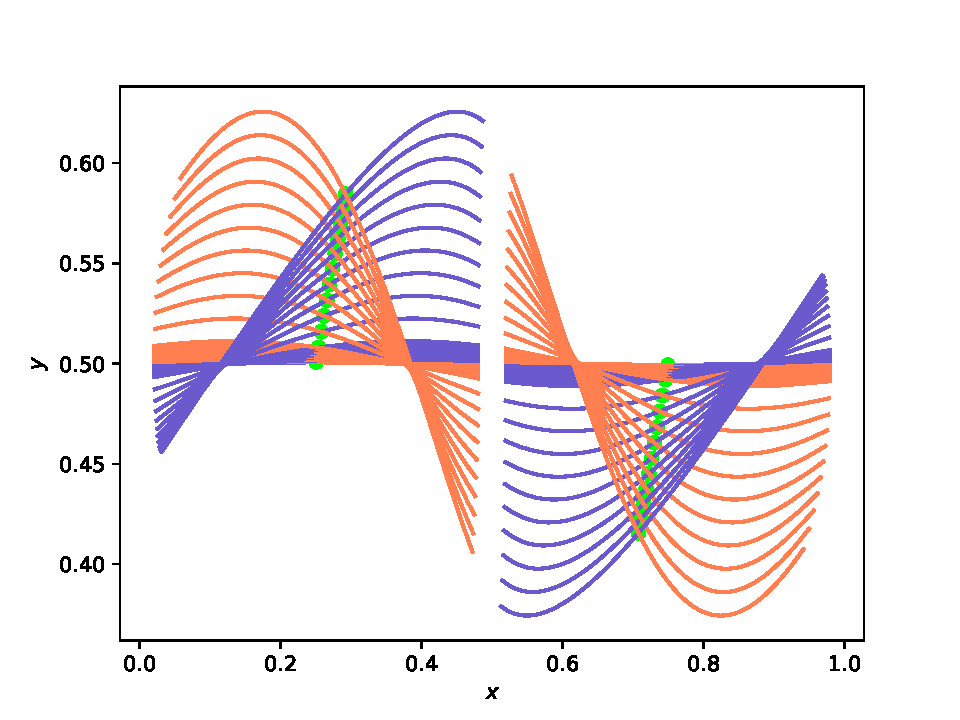
\includegraphics[scale=0.5]{variedadesestandarkappas}
	\caption{Comportamiento de las variedades invariantes asociadas a la \'orbita de periodo dos en el mapeo est\'andar al variar $\kappa$ entre $[0.1,1.1]$.}
	\label{variedadesestandarkappasv}
\end{figure}

\begin{figure}[H]
	\centering
	\includegraphics[scale=0.5]{variedadesestperiodo3kvar}
	\caption{Variedades asociadas a una \'orbita de periodo tres para el mapeo est\'andar con valores de $\kappa = [0.01,0.02,0.03]$. }
	\label{vairedadesperiodo3kvariable}
\end{figure}

\begin{figure}[H]
	\centering
	\includegraphics[scale=0.7]{variedadesestandarperiodo3}
	\caption{Variedades invariantes asociadas a una \'orbita de periodo tres en el mapeo est\'andar con diferentes valores de $\kappa$.}
	\label{variedadesestandarperiodo3}
\end{figure}
\begin{figure}[H]
	\centering
	\includegraphics[scale=0.7]{erroresvariedadesestandarperiodo3}
	\caption{Errores asociados al c\'alculo de las variedades invariantes de la figura \ref{variedadesestandarperiodo3}. }
	\label{erroresvariedadesperiodo3}
\end{figure}

\begin{figure}[H]
	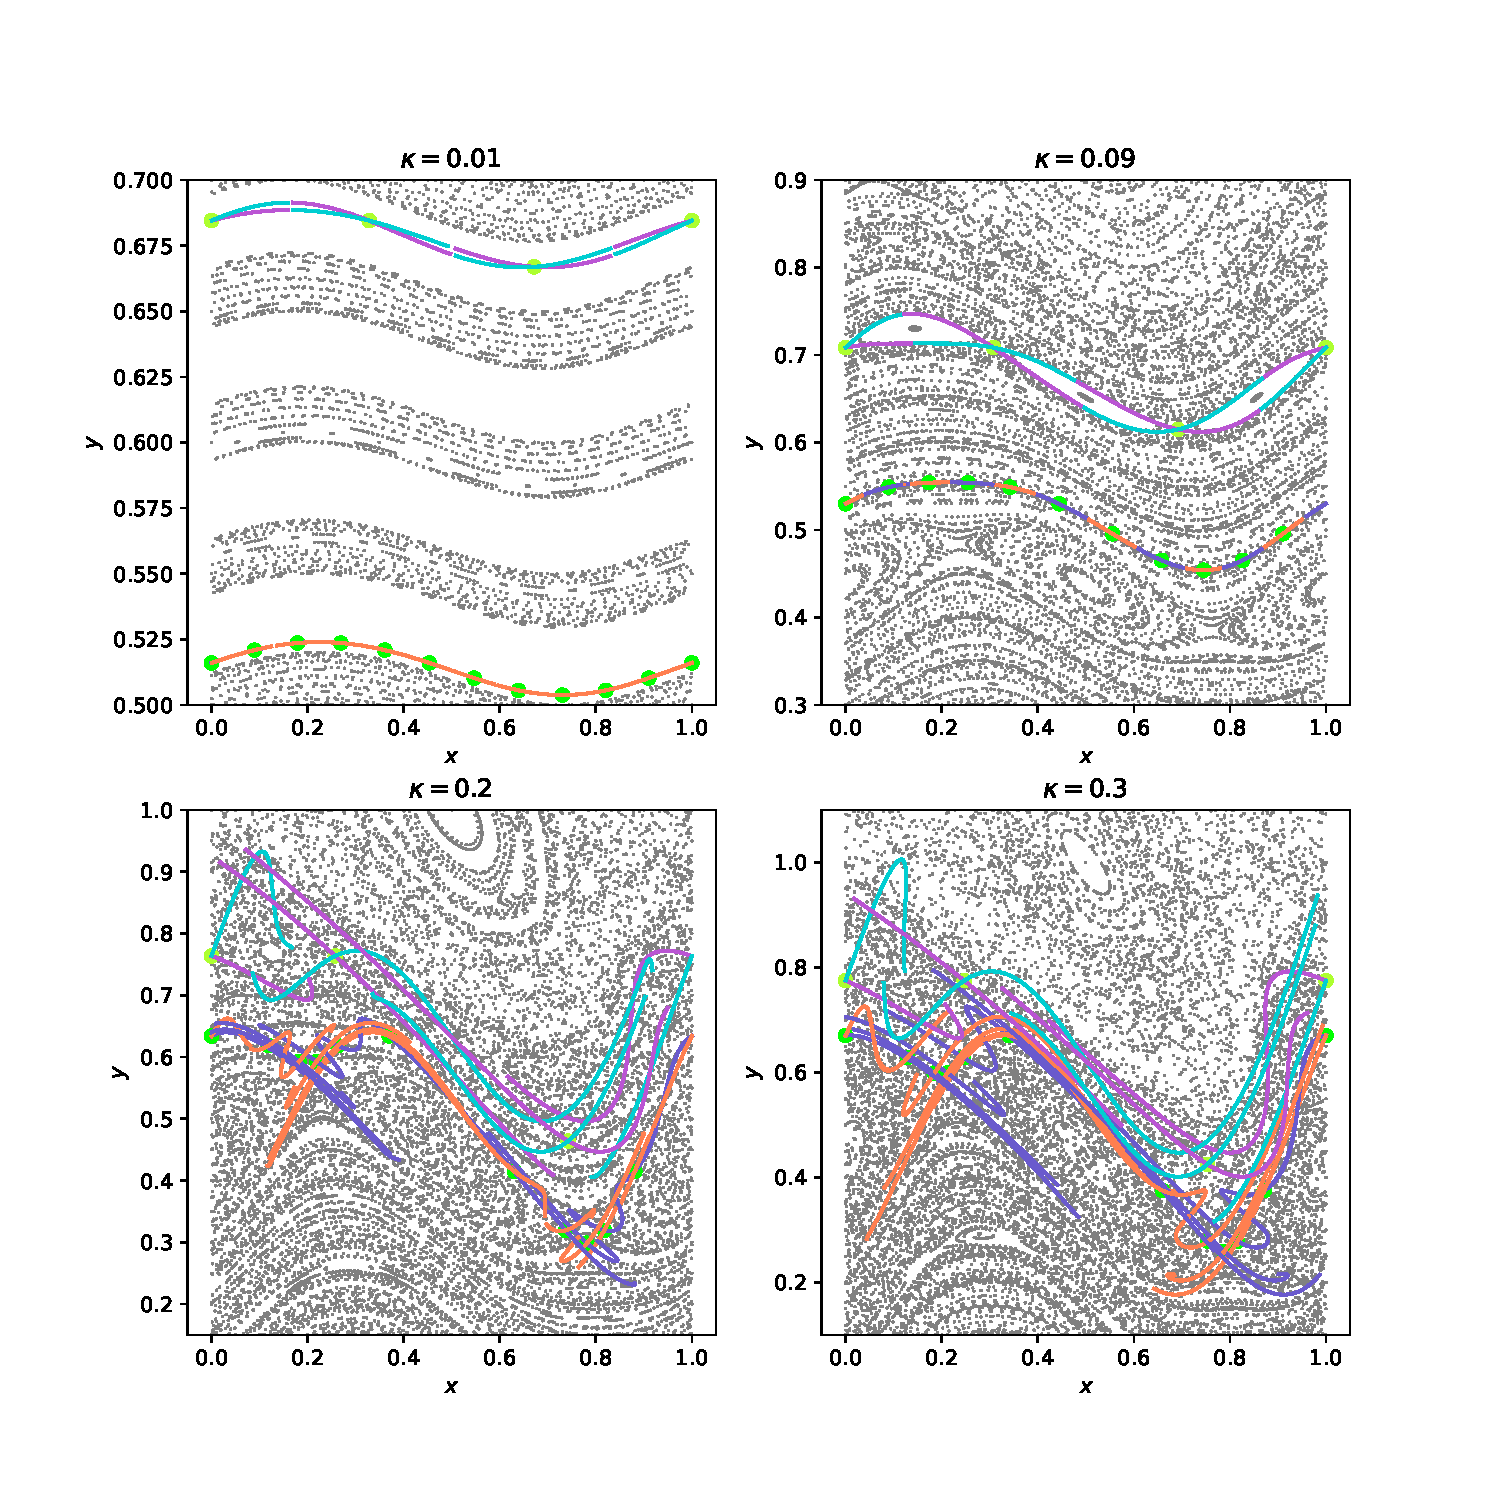
\includegraphics[scale=0.7]{variedadescuadraticop3p11A}
	\caption{Variedades invariantes asociadas a dos \'orbitas de periodo tres y once respectivamente, para el mapeo \eqref{mapeocuadratico}, con diferentes valores del par\'ametro $b$ y manteniendo $a=0.618$ fijo.}
	\label{variedadescuadraticoper3per11vark}
\end{figure}
\section{Conclusiones}
Mediante el m\'etodo descrito para encontrar \'orbitas peri\'odicas es posible encontrar \'orbitas de periodo $N$ en mapeos simpl\'ecticos de dos dimensiones usando una semilla adecuada y siempre que se cuente con las involuciones. Dado que el m\'etodo usa internamente un m\'etodo para encontrar ra\'ices en una dimensi\'on es importante tener en cuenta que se cumplan los requerimentos para que el m\'etodo num\'erico converja. Las instrucciones de c\'omo puede modificarse el m\'etodo o la presici\'on con la que se calculan las \'orbitas puede encontrarse en \url{https://github.com/alvarezeve/PeriodicOrbits2DMaps}. \\

Se present\'o adem\'as una forma para determinar la estabilidad de las \'orbitas encontradas. Esta f\'ormula proviene de usar la regla de la cadena en la composici\'on del mapeo con el que se est\'e trabajando y del hecho de que cualquier \'orbita de periodo $N$ es un punto fijo del mapeo $M^{N}$. Usando esto y la forma en la que se determina la estabilidad de un punto fijo se implement\'o una forma f\'acil para determinar la estabilidad.\\

Para las \'orbitas peri\'odicas hiperb\'olicas se aplic\'o el m\'etodo de la parametrizaci\'on para describir las variedades asociadas. El m\'etodo ya hab\'ia sido implementado previamente para puntos fijos hiperb\'olicos de mapeos de dos dimensiones por lo que solo fueron necesarios algunas modificaciones simples para usarlo en \'orbitas peri\'odicas. Mediante este m\'etodo fue posible describir el comportamiendo de variedades asociadas a \'orbitas per\'iodicas en cada uno de los puntos de la \'orbita.\\

El orden de la parametrizaci\'on se puede elegir y modificar para que la variedad se pueda describir con un error aceptable en alg\'un intervalo deseado. Sin embargo no es posible con solo aumentar el orden del polinomio describir una variedad en intervalos \textit{grandes} (el tamaño depende del mapeo y de la \'orbita peri\'odica), por lo que una alternativa es aplicar el mapeo a la parametrizaci\'on, como una especie de iteraci\'on pero no de puntos en el espacio fase, sino directamente de la expresi\'on polin\'omica de la variedad. La iteraci\'on de la variedad nos da un nuevo polinomio con diferentes coeficientes que pueden describir un intervalo mayor de la variedad. \\

Uniendo los m\'etodos fue posible observar la din\'amica de las \'orbitas peri\'odicas y de las variedades asociadas cuando el par\'ametro $\kappa$ en el mapeo est\'andar, o el par\'ametro $b$ en el mapeo \eqref{mapeocuadratico} van increment\'andose. 






